
\begin{figure}[H]
  \begin{center}
    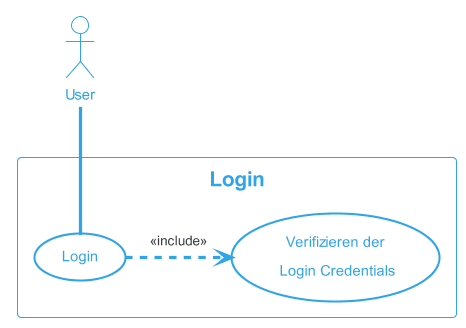
\includegraphics[width=0.6\linewidth]{content/diagrams/out/usecase/login/Login.png}
    \caption{UC-Login}
    \label{login}
  \end{center}
\end{figure}

\begin{table}[H]
  \newcolumntype{a}{>{\columncolor[HTML]{4473C5}}L}
  \centering
  \settowidth\tymin{\textbf{Kurzbeschreibung}}
  \setlength\extrarowheight{2pt}
  \begin{tabulary}{1.0\textwidth}{|a|m{14cm}|}
    \hline
    \textbf{Name}& Login\\
    \hline
    \textbf{Akteur}& Mitarbeiter:in der Liegenschaftsverwaltung, Hauswartungspersonen, Geschäftsführer\\
    \hline 
    \textbf{Beschreibung} & Ein Akteur will sich in der Applikation anmelden\\
    \hline
    \textbf{Daten} & Login-Daten des Benutzers\\
    \hline
    \textbf{Auslöser} & Benutzerbefehl der von dem entsprechenden Akteur initiiert wird\\
    \hline
    \textbf{Antwort} & Bestätigung, dass das Login erfolgreich war\\
    \hline
    \textbf{Kommentare} & -\\
    \hline
  \end{tabulary}
  \caption{UC-Login}
\end{table}

\begin{figure}[H]
  \begin{center}
    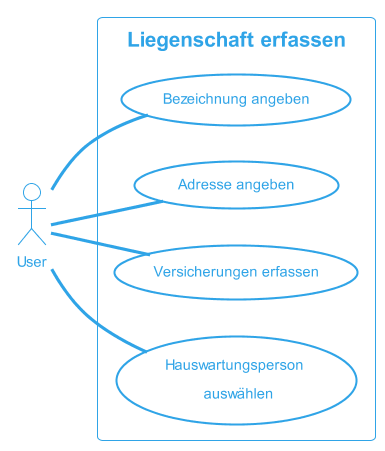
\includegraphics[width=0.43\linewidth]{content/diagrams/out/usecase/liegenschaftErfassen/LiegenschaftErfassen.png}
    \caption{UC-Liegenschaft erfassen}
    \label{Liegenschaft}
  \end{center}
\end{figure}

\vspace*{-1cm}

\begin{table}[H]
  \newcolumntype{a}{>{\columncolor[HTML]{4473C5}}L}
  \centering
  \settowidth\tymin{\textbf{Kurzbeschreibung}}
  \setlength\extrarowheight{2pt}
  \begin{tabulary}{1.0\textwidth}{|a|m{14cm}|}
    \hline
    \textbf{Name}& Liegenschaft erfassen\\
    \hline
    \textbf{Akteur}& Mitarbeiter:in der Liegenschaftsverwaltung\\
    \hline 
    \textbf{Beschreibung} & Der zuständige Mitarbeiter:in loggt sich in der Applikation ein und kann anschliessend die Liegenschaft über einen Button erfassen. Es müssen alle Daten zur Liegenschaft eingetragen werden sonst kann der Mitarbeiter die Liegenschaft nicht abspeichern.\\
    \hline
    \textbf{Daten} & Informationen zur Liegenschaft\\
    \hline
    \textbf{Auslöser} & Benutzerbefehl der von dem entsprechenden Akteur initiiert wird\\
    \hline
    \textbf{Antwort} & Bestätigung, dass das erfassen der Liegenschaft erfolgreich war\\
    \hline
    \textbf{Kommentare} & Bei fehlenden Angaben wird dem Benutzer eine Fehlermeldung angezeigt\\
    \hline
  \end{tabulary}
  \caption{UC-Liegenschaft erfassen}
\end{table}

\begin{figure}[H]
  \begin{center}
    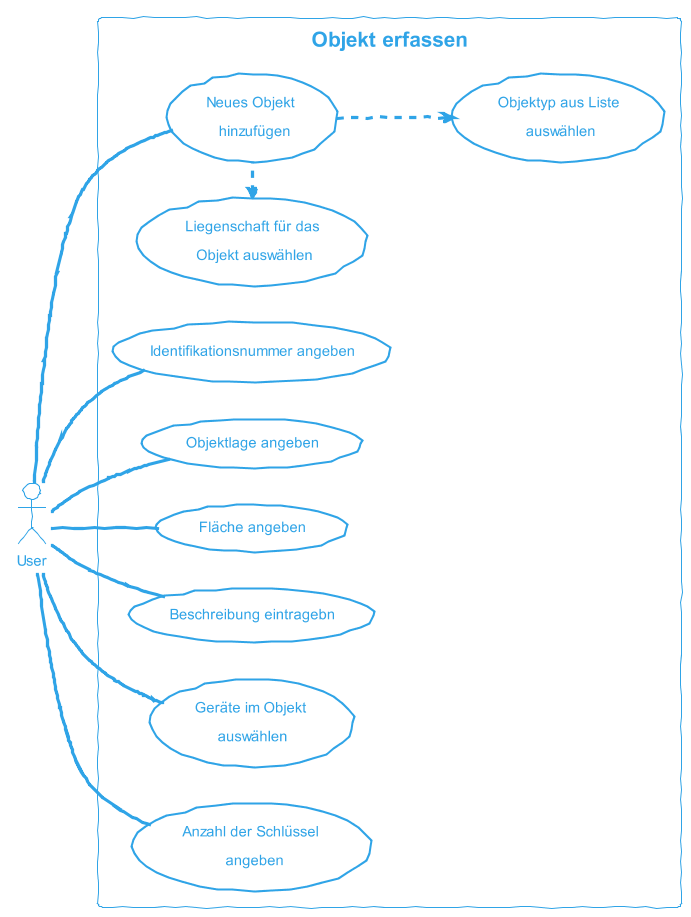
\includegraphics[width=0.8\linewidth]{content/diagrams/out/usecase/objektErfassen/ObjektErfassen.png}
    \caption{UC-Objekt erfassen}
    \label{objekt}
  \end{center}
\end{figure}

\vspace*{-1cm}

\begin{table}[H]
  \newcolumntype{a}{>{\columncolor[HTML]{4473C5}}L}
  \centering
  \settowidth\tymin{\textbf{Kurzbeschreibung}}
  \setlength\extrarowheight{2pt}
  \begin{tabulary}{1.0\textwidth}{|a|m{14cm}|}
    \hline
    \textbf{Name}& Objekt erfassen\\
    \hline
    \textbf{Akteur}& Mitarbeiter:in der Liegenschaftsverwaltung\\
    \hline 
    \textbf{Beschreibung} & Der zuständige Mitarbeiter:in loggt sich in der Applikation ein und kann anschliessend das Objekt über einen Button erfassen. Es müssen alle Daten zum Objekt eingetragen werden sonst kann dieses nicht abgespeichert werden\\
    \hline
    \textbf{Daten} & Informationen zum Objekt\\
    \hline
    \textbf{Auslöser} & Benutzerbefehl der von dem entsprechenden Akteur initiiert wird\\
    \hline
    \textbf{Antwort} & Bestätigung, dass das erfassen des Objektes erfolgreich war\\
    \hline
    \textbf{Kommentare} & Bei fehlenden Angaben wird dem Benutzer eine Fehlermeldung angezeigt\newline 
    Ein Objekt kann nur über eine Liegenschaft erfasst werden\\
    \hline
  \end{tabulary}
  \caption{UC-Objekt erfassen}
\end{table}

\begin{figure}[H]
  \begin{center}
    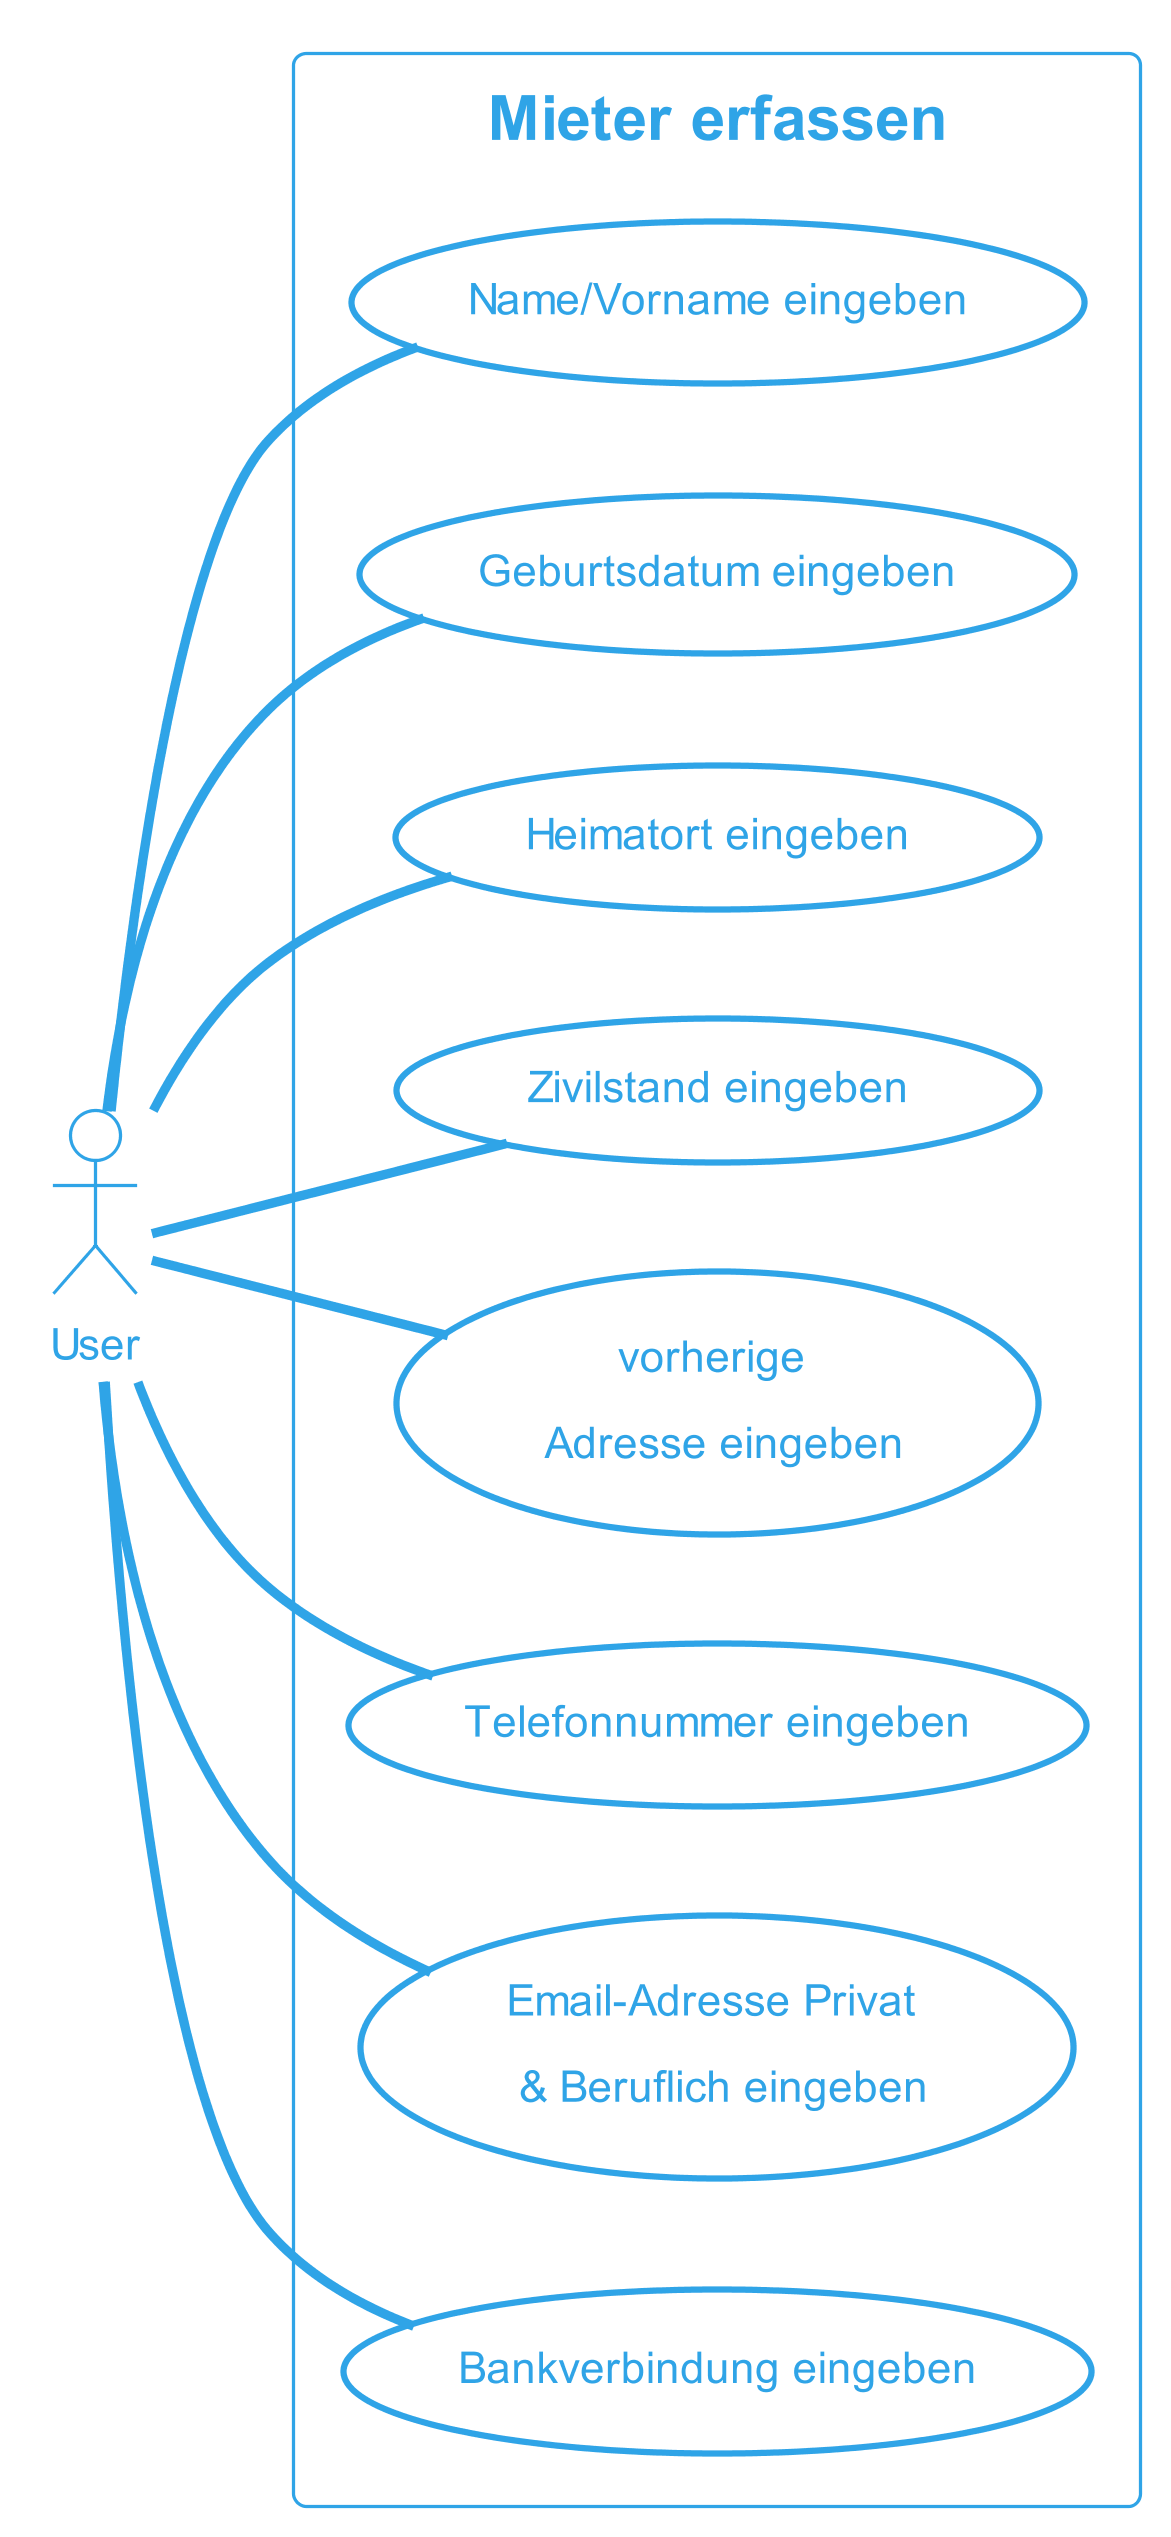
\includegraphics[width=0.4\linewidth]{content/diagrams/out/usecase/mieterErfassen/Mieter erfassen.png}
    \caption{UC-Mieter:in erfassen}
    \label{mieterErfassen}
  \end{center}
\end{figure}

\begin{table}[H]
  \newcolumntype{a}{>{\columncolor[HTML]{4473C5}}L}
  \centering
  \settowidth\tymin{\textbf{Kurzbeschreibung}}
  \setlength\extrarowheight{2pt}
  \begin{tabulary}{1.0\textwidth}{|a|m{14cm}|}
    \hline
    \textbf{Name}& Mieter:in erfassen\\
    \hline
    \textbf{Akteur}& Mitarbeiter:in der Liegenschaftsverwaltung\\
    \hline 
    \textbf{Beschreibung} & Wird die Bewerbung eines Mieters für ein Objekt angenommen, muss dieser Mieter:in in der Applikation erfasst werden. Der zuständige Mitarbeiter:in loggt sich dazu in der Applikation ein und kann den Mieter:in im entsprechenden Formular erfassen\\
    \hline
    \textbf{Daten} & Vollständige Daten zum Mieter\\
    \hline
    \textbf{Auslöser} & Benutzerbefehl der von dem entsprechenden Akteur initiiert wird\\
    \hline
    \textbf{Antwort} & Bestätigung, dass der Mieter erfolgreich erfasst wurde\\
    \hline
    \textbf{Kommentare} & -\\
    \hline
  \end{tabulary}
  \caption{UC-Mieter:in erfassen}
\end{table}

\begin{figure}[H]
  \begin{center}
    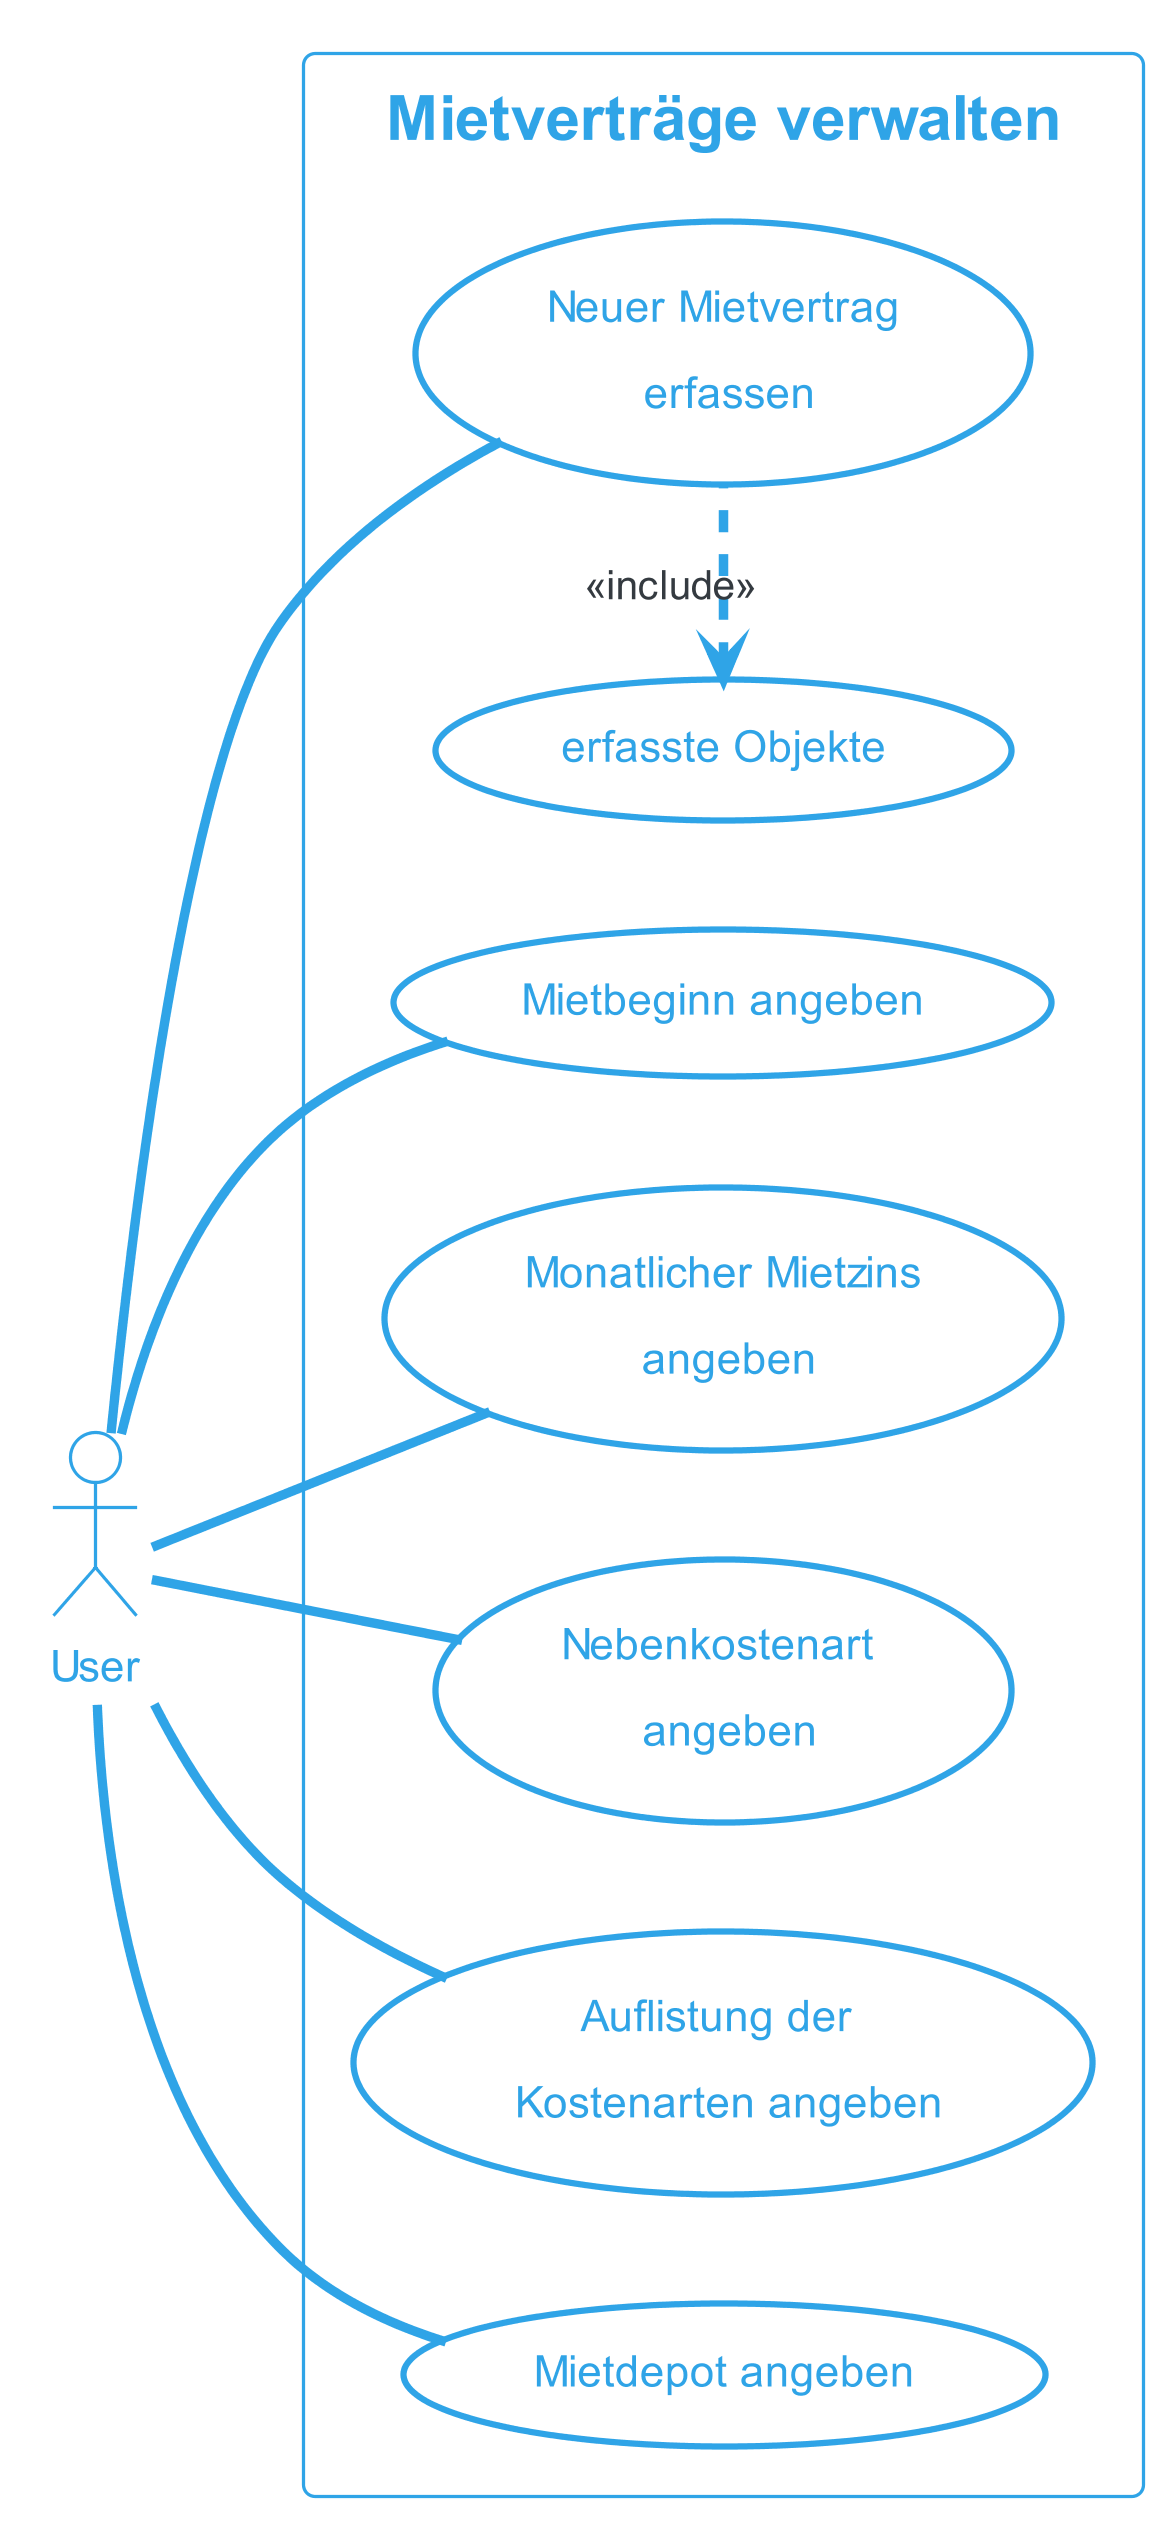
\includegraphics[width=0.43\linewidth]{content/diagrams/out/usecase/mietverträgeVerwalten/MietverträgeVerwalten.png}
    \caption{UC-Mietverträge verwalten}
    \label{MietvertraegeVerwalten}
  \end{center}
\end{figure}

\vspace*{-1cm}

  \begin{table}[H]
    \newcolumntype{a}{>{\columncolor[HTML]{4473C5}}L}
    \centering
    \settowidth\tymin{\textbf{Kurzbeschreibung}}
    \setlength\extrarowheight{2pt}
      \begin{tabulary}{1.0\textwidth}{|a|m{14cm}|}
        \hline
        \textbf{Name}& Mietverträge verwalten\\
      \hline
      \textbf{Akteur}& Mitarbeiter:in der Liegenschaftsverwaltung\\
      \hline 
      \textbf{Beschreibung} & Der zuständige Mitarbeiter:in loggt sich in der Applikation ein und erstellt anschliessend einen neuen Mietvertrag der noch den Status ungültig hat, bis dieser von beiden Parteien unterschrieben wurde\\
      \hline
      \textbf{Daten} & Alle Daten die zum erfassen des Mietvertrags nötig sind \\
      \hline
      \textbf{Auslöser} & Benutzerbefehl der von dem entsprechenden Akteur initiiert wird\\
      \hline
      \textbf{Antwort} & Bestätigung, dass der Mietvertrag erfolgreich erfasst wurde und ausgedruckt werden kann\\
      \hline
      \textbf{Kommentare} & Bei fehlenden Angaben wird dem Benutzer eine Fehlermeldung angezeigt\\
      \hline
  \end{tabulary}
  \caption{UC-Mietverträge verwalten}
  \end{table}

\begin{figure}[H]
  \begin{center}
    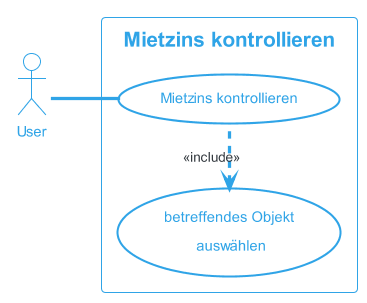
\includegraphics[width=0.4\linewidth]{content/diagrams/out/usecase/mietzinsKontrollieren/MietzinsKontrollieren.png}
    \caption{UC-Mietzins kontrollieren}
    \label{MietzinsKontrollieren}
  \end{center}
\end{figure}

\begin{table}[H]
  \newcolumntype{a}{>{\columncolor[HTML]{4473C5}}L}
  \centering
  \settowidth\tymin{\textbf{Kurzbeschreibung}}
  \setlength\extrarowheight{2pt}
  \begin{tabulary}{1.0\textwidth}{|a|m{14cm}|}
    \hline
    \textbf{Name}& Mietzins kontrollieren\\
    \hline
    \textbf{Akteur}& Mitarbeiter:in der Liegenschaftsverwaltung\\
    \hline 
    \textbf{Beschreibung} & Wenn die Zahlungen geprüft werden müssen, loggt sich der zuständige Mitarbeiter:in ein und kann auf dem entsprechenden Objekt Kontrollieren ob die Miete oder die Nebenkosten schon als ''bezahlt'' markiert wurde\\
    \hline
    \textbf{Daten} & Zu prüfendes Objekt\\
    \hline
    \textbf{Auslöser} & Benutzerbefehl der von dem entsprechenden Akteur initiiert wird\\
    \hline
    \textbf{Antwort} & Zahlungen wurde getätigt oder im Verzug\\
    \hline
    \textbf{Kommentare} & Bei Zahlungen im Verzug wird der nächste UseCase \fref{mahnung} eingesetzt\\
    \hline
  \end{tabulary}
  \caption{UC-Mietzins kontrollieren}
\end{table}

\newpage

\begin{figure}[H]
  \begin{center}
    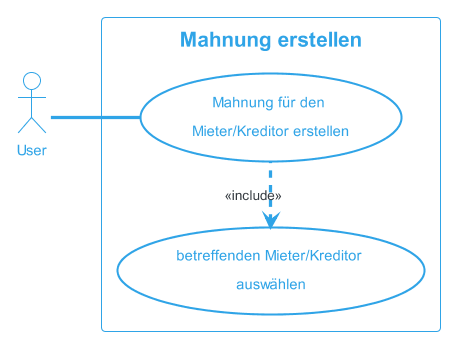
\includegraphics[width=0.5\linewidth]{content/diagrams/out/usecase/mahnungGenerieren/MahnungErstellen.png}
    \caption{UC-Mahnung erstellen}
    \label{mahnung}
  \end{center}
\end{figure}

\begin{table}[H]
  \newcolumntype{a}{>{\columncolor[HTML]{4473C5}}L}
  \centering
  \settowidth\tymin{\textbf{Kurzbeschreibung}}
  \setlength\extrarowheight{2pt}
  \begin{tabulary}{1.0\textwidth}{|a|m{14cm}|}
    \hline
    \textbf{Name}& Mahnung erstellen\\
    \hline
    \textbf{Akteur}& Mitarbeiter:in der Liegenschaftsverwaltung\\
    \hline 
    \textbf{Beschreibung} & Fällt die Prüfung der Mietzins-oder Nebenkostenzahlung negativ aus, kann der Benutzer eine Mahnung für den Mieter erstellen \\
    \hline
    \textbf{Daten} & Rechnungsbetrag\\
    \hline
    \textbf{Auslöser} & Benutzerbefehl der von dem entsprechenden Akteur initiiert wird\\
    \hline
    \textbf{Antwort} & Bestätigung, dass die Mahnung erfolgreich erstellt wurde und jetzt ausgedruckt werden kann\\
    \hline
    \textbf{Kommentare} & Normalerweise ist der zuständige Mitarbeiter:in in der Applikation schon eingeloggt da er die Prüfung der Zahlung vorgenommen hatte. Das erstellen der Mahnung wird dann direkt von dort aus ausgelöst\\
    \hline
  \end{tabulary}
  \caption{UC-Mahnung erstellen}
\end{table}

\begin{figure}[H]
  \begin{center}
    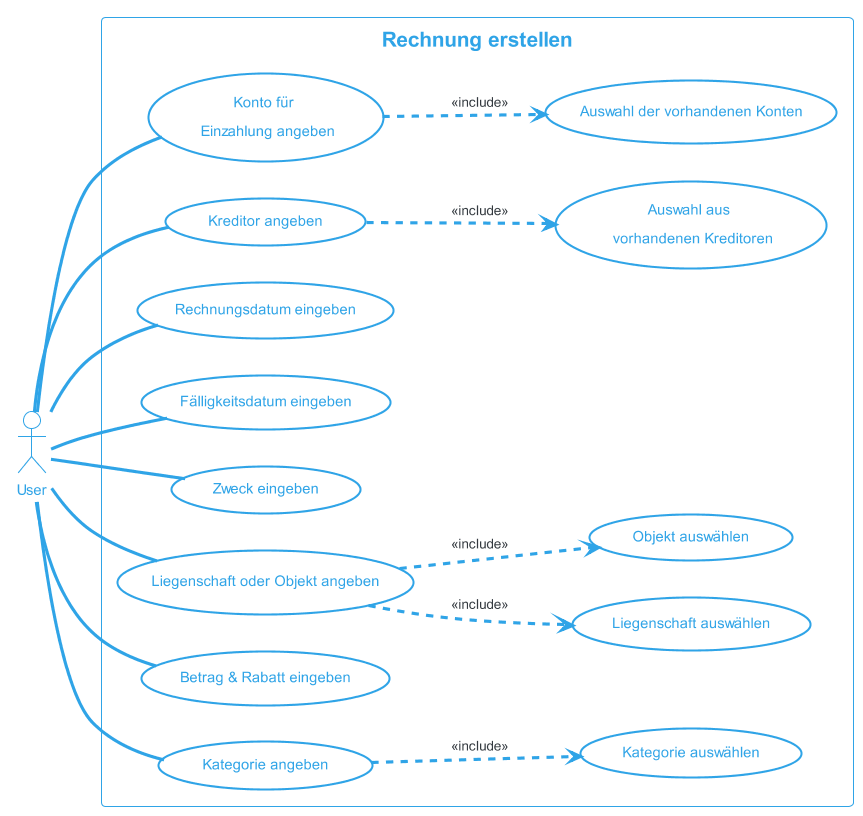
\includegraphics[width=0.85\linewidth]{content/diagrams/out/usecase/rechnungErstellen/Rechnung erstellen.png}
    \caption{UC-Rechnung erstellen}
    \label{RechnungErstellen}
  \end{center}
\end{figure}
\vspace*{-1.2cm}
\begin{table}[H]
  \newcolumntype{a}{>{\columncolor[HTML]{4473C5}}L}
  \centering
  \settowidth\tymin{\textbf{Kurzbeschreibung}}
  \setlength\extrarowheight{2pt}
  \begin{tabulary}{1.0\textwidth}{|a|m{14cm}|}
    \hline
    \textbf{Name}& Rechnung erstellen\\
    \hline
    \textbf{Akteur}& Mitarbeiter:in der Liegenschaftsverwaltung\\
    \hline 
    \textbf{Beschreibung} & Um eine Rechnung zu erstellen, muss sich der Zuständige Mitarbeiter:in in der Applikation einloggen. Es kann dann für eine Dienstleistung eine Rechnung erstellt werden. Um die Rechnung für eine Dienstleistung zu erstellen, müssen alle Daten eingegeben werden \newline 
    Wird eine Rechnung für die fällige Miete oder die Nebenkosten erstellt, werden die Daten für die Rechnung aus der angewählten Liegenschaft oder Objekt in die Rechnung eingefügt. Allfällige Anpassungen können nachträglichen als separate Rechnungsposition hinzugefügt werden \newline
    Die Rechnungen werden immer einem Konto zugeordnet. Falls das gewünschte Konto noch nicht besteht, muss es noch erstellt werden\\
    \hline
    \textbf{Daten} &       
      $\bullet$ Kreditor\newline
      $\bullet$ Rechnungsbetrag \newline
      $\bullet$ Objekt oder Liegenschaft\\
    \hline
    \textbf{Auslöser} & Benutzerbefehl der von dem entsprechenden Akteur initiiert wird\\
    \hline
    \textbf{Antwort} & Bestätigung, dass die Rechnung erfolgreich erstellt wurde und ausgedruckt werden kann\\
    \hline
    \textbf{Kommentare} & Falls der Kreditor oder das Konto noch nicht erfasst wurde, muss dies noch gemacht werden. Siehe UseCase \hyperref[kreditorErfassen]{Kreditor Erfassen \fref{kreditorErfassen}} bzw. \hyperref[kreditorErfassen]{Kreditor Erfassen \fref{kreditorErfassen}}\\
    \hline
  \end{tabulary}
  \caption{UC-Rechnung erstellen}
\end{table}

\begin{figure}[H]
  \begin{center}
      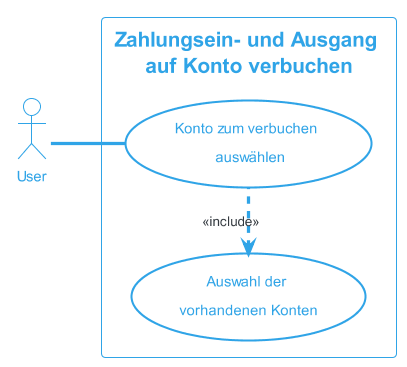
\includegraphics[width=0.5\linewidth]{content/diagrams/out/usecase/verbuchenAufKonto/ZahlungseingangaufKontoverbuchen.png}
    \caption{UC-Zahlungseingang auf Konto verbuchen}
    \label{ZahlungaufKonto}
  \end{center}
\end{figure}

\begin{table}[H]
  \newcolumntype{a}{>{\columncolor[HTML]{4473C5}}L}
  \centering
  \settowidth\tymin{\textbf{Kurzbeschreibung}}
  \setlength\extrarowheight{2pt}
  \begin{tabulary}{1.0\textwidth}{|a|m{14cm}|}
    \hline
    \textbf{Name}& Zahlungsein- und Ausgang auf Konto verbuchen\\
    \hline
    \textbf{Akteur}& Mitarbeiter:in der Liegenschaftsverwaltung\\
    \hline 
    \textbf{Beschreibung} & Bei einem Zahlungseingang, muss dieser auf ein entsprechendes Konto verbucht werden. Normalerweise gibt es aufgrund einer gestellten Rechnung einen Zahlungseingang. Wenn die Rechnung als bezahlt markiert wird, wird der Zahlungseingang auf das mit der Rechnung verknüpfte Konto verbucht \newline
    Falls es einen Zahlungsein- oder Ausgang gibt der nicht aufgrund einer Rechnung geschieht, muss dieser Eintrag manuell für das entsprechende Konto erstellt werden\\
    \hline
    \textbf{Daten} & Rechnungsnummer oder Zahlungsbetrag und Konto\\
    \hline
    \textbf{Auslöser} & Zahlungseingang\\
    \hline
    \textbf{Antwort} & Bestätigung, dass der Zahlungseingang verbucht wurde\\
    \hline
    \textbf{Kommentare} & Wenn das Konto zu dem der Zahlungsein- oder Ausgang erfasst werden soll noch nicht besteht, muss dies noch erstellt werden. Siehe \hyperref[kontoErstellen]{Konto erstellen \fref{kontoErstellen}}\\
    \hline
  \end{tabulary}
  \caption{UC-Zahlungsein- und Ausgang auf Konto verbuchen}
\end{table}

\newpage
\begin{figure}[H]
  \begin{center}
    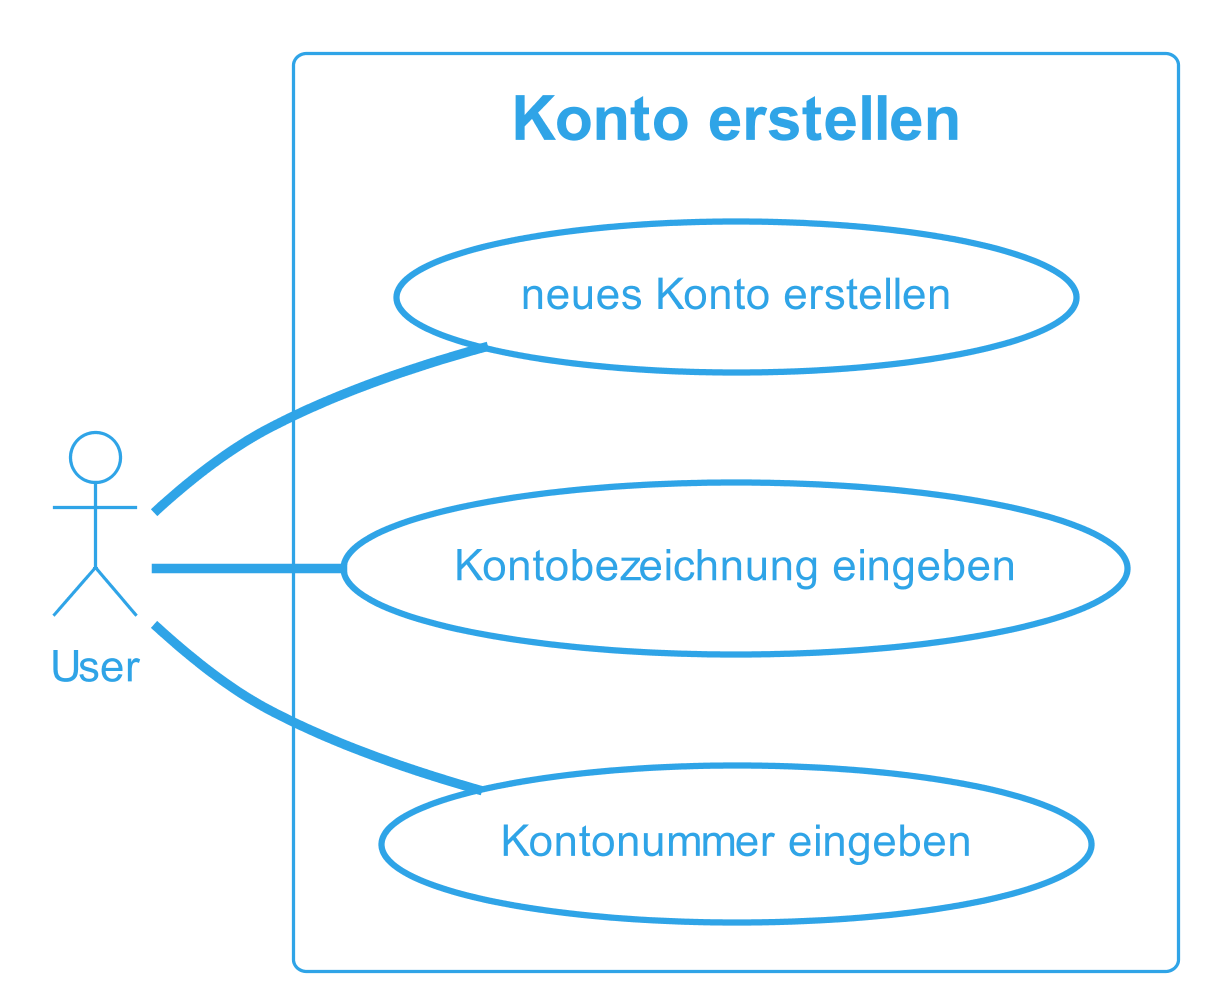
\includegraphics[width=0.5\linewidth]{content/diagrams/out/usecase/kontoErstellen/kontoErstellen.png}
    \caption{UC-Konto erstellen}
    \label{kontoErstellen}
  \end{center}
\end{figure}

\begin{table}[H]
  \newcolumntype{a}{>{\columncolor[HTML]{4473C5}}L}
  \centering
  \settowidth\tymin{\textbf{Kurzbeschreibung}}
  \setlength\extrarowheight{2pt}
  \begin{tabulary}{1.0\textwidth}{|a|m{14cm}|}
    \hline
    \textbf{Name}& Konto erstellen\\
    \hline
    \textbf{Akteur}& Mitarbeiter:in der Liegenschaftsverwaltung\\
    \hline 
    \textbf{Beschreibung} & Ein neues Konto zum verbuchen Der Zahlungen muss erstellt werden\\
    \hline
    \textbf{Daten} & Kontobezeichnung und Kontonummer\\
    \hline
    \textbf{Auslöser} & Benutzerbefehl, der von dem entsprechenden Akteur initiiert wird\\
    \hline
    \textbf{Antwort} & Bestätigung, dass das Konto erfolgreich erstellt wurde\\
    \hline
    \textbf{Kommentare} & -\\
    \hline
  \end{tabulary}
  \caption{UC-Konto erstellen}
\end{table}

\begin{figure}[H]
  \begin{center}
    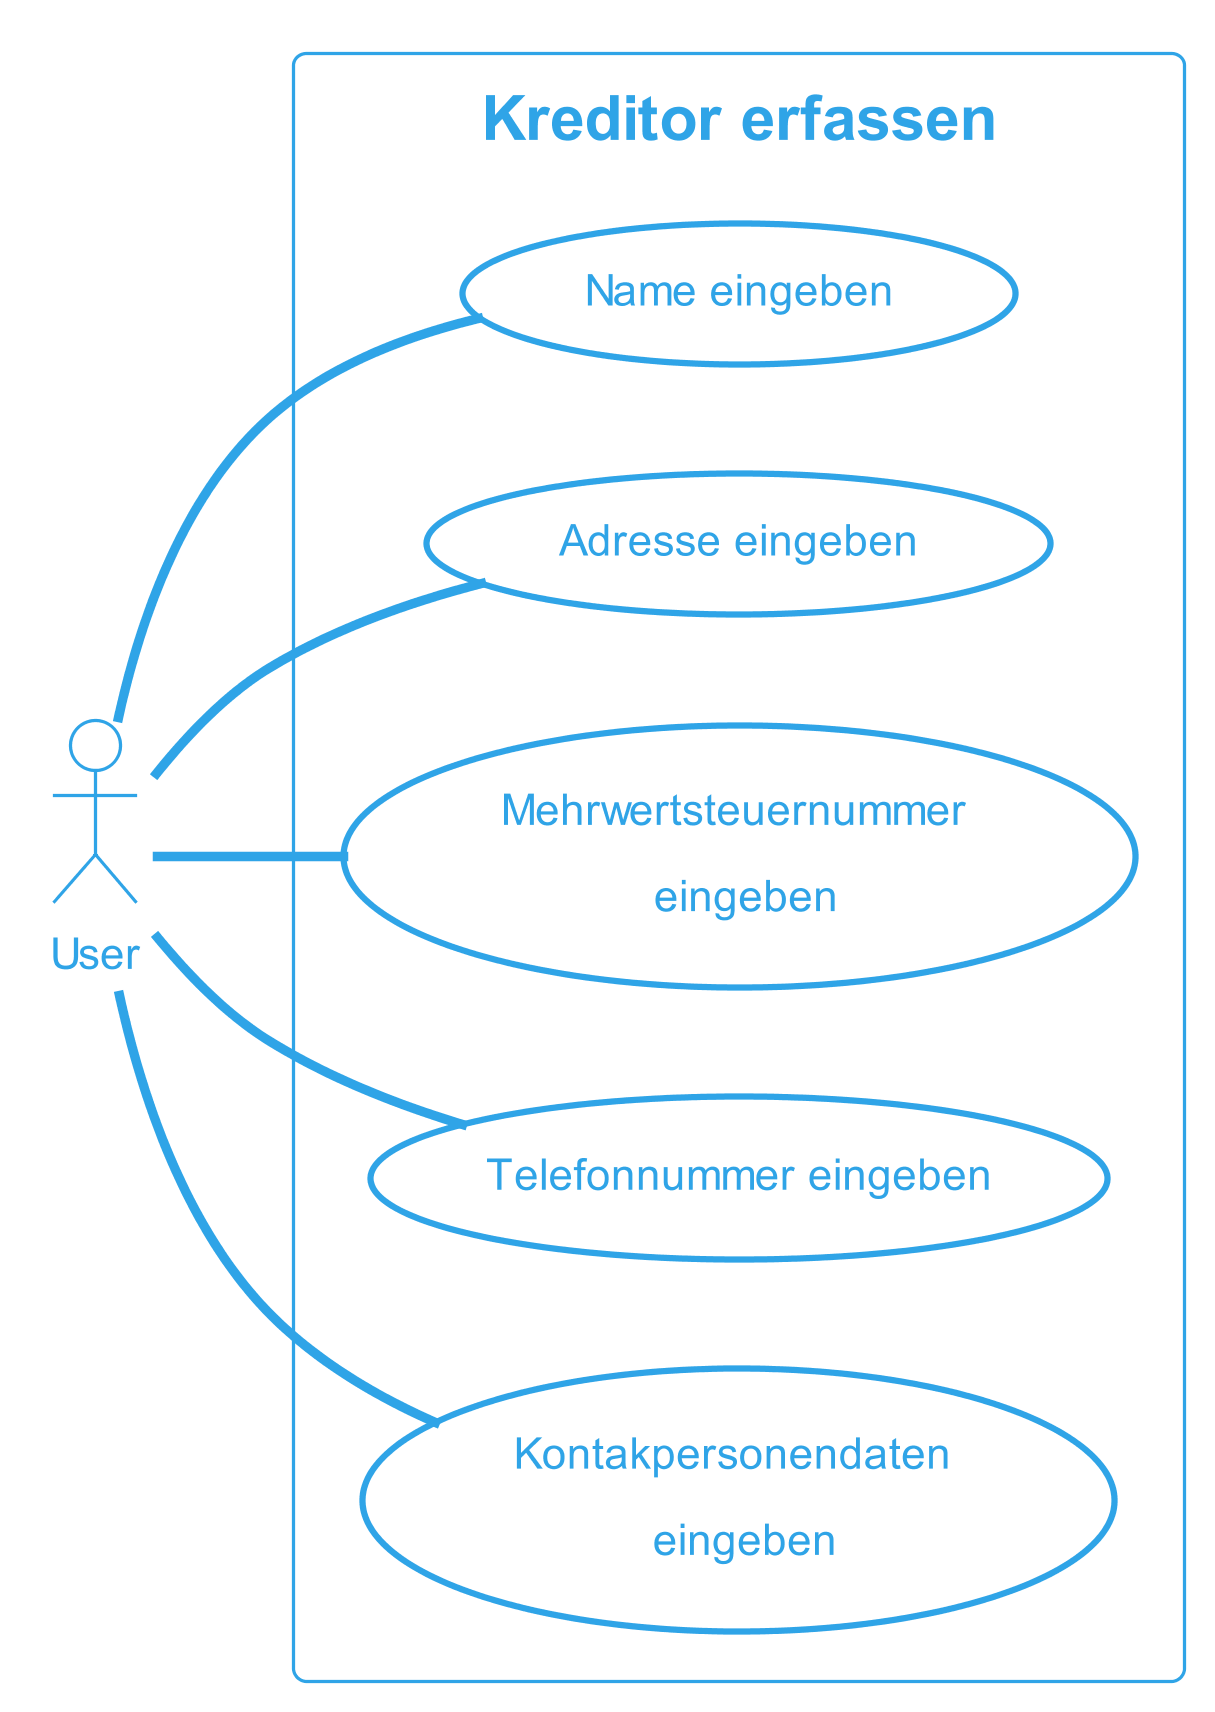
\includegraphics[width=0.5\linewidth]{content/diagrams/out/usecase/kreditorErfassen/Kreditor erfassen.png}
    \caption{UC-Kreditor erfassen}
    \label{kreditorErfassen}
  \end{center}
\end{figure}

\begin{table}[H]
  \newcolumntype{a}{>{\columncolor[HTML]{4473C5}}L}
  \centering
  \settowidth\tymin{\textbf{Kurzbeschreibung}}
  \setlength\extrarowheight{2pt}
  \begin{tabulary}{1.0\textwidth}{|a|m{14cm}|}
    \hline
    \textbf{Name}& Kreditor erfassen\\
    \hline
    \textbf{Akteur}& Mitarbeiter:in der Liegenschaftsverwaltung\\
    \hline 
    \textbf{Beschreibung} & Wir für einen Kreditor eine Rechnung erstellt der noch nicht erfasst wurde, wird dies hier gemacht\\
    \hline
    \textbf{Daten} & Vollständige Daten zum Kreditor\\
    \hline
    \textbf{Auslöser} & Benutzerbefehl der von dem entsprechenden Akteur initiiert wird\\
    \hline
    \textbf{Antwort} & Bestätigung, dass der Kreditor erfolgreich erfasst wurde\\
    \hline
    \textbf{Kommentare} & Normalwerkweise ist der Benutzer in der Applikation schon eingeloggt, weil erst beim erstellen der Rechnung bemerkt wird, dass der Kreditor noch nicht erfasst wurde. Für Miet-und Nebenkostenabrechnungen sind die Mieter die Kreditoren \\
    \hline
  \end{tabulary}
  \caption{UC-Kreditor erfassen}
\end{table}
